\documentclass[a4paper, 10pt]{article}
\usepackage{helvet}
\renewcommand{\familydefault}{\sfdefault}
\usepackage{pgf}
\usepackage{eurosym}
\usepackage{graphicx}
\usepackage{wasysym}
\usepackage{hyperref}
\usepackage{listings}
\usepackage{pxfonts}
\usepackage{verbatim}
\usepackage{color}
\usepackage{xcolor}
\usepackage{wrapfig}
\usepackage{enumitem}
\usepackage{booktabs}
\usepackage{gensymb}
\usepackage{tabularx}
\usepackage{currfile}

\hypersetup{
    bookmarks=true,         % show bookmarks bar?
    unicode=true,          % non-Latin characters in Acrobat’s bookmarks
    pdftoolbar=true,        % show Acrobat’s toolbar?
    pdfmenubar=true,        % show Acrobat’s menu?
    pdffitwindow=true,     % window fit to page when opened
    pdftitle={Assessments},    % title
    pdfauthor={Paul Vesey},     % author
    pdfsubject={I.C.T. Building Information Modelling},   % subject of the document
    pdfcreator={},   % creator of the document
    pdfproducer={xelatex}, % producer of the document
    pdfkeywords={'Graphics' }, % list of keywords
    pdfnewwindow=true,      % links in new PDF window
    colorlinks=true,       % false: boxed links; true: colored links
    linkcolor=violet,          % color of internal links (change box color with linkbordercolor)
    citecolor=magenta,        % color of links to bibliography
    filecolor=red,      % color of file links
    urlcolor=blue           % color of external links
}

\setlength\parindent{0pt}
\begin{document}

\lstset{language=HTML,
				basicstyle=\small,
				breaklines=true,
        numbers=left,
        numberstyle=\tiny,
        showstringspaces=false,
        aboveskip=-20pt,
        frame=leftline
        }
				
\begin{figure}
	\centering
	
\includegraphics[width=0.5\linewidth]{./Assignments/img/LITlogo}
\end{figure}


\begin{tabularx}{\textwidth}{ |l|X| }
	\hline
	\textbf{Subject:} & COMP06051-ICT \& BIM\\
	\textbf{Course:} & BEng in Civil Engineering\\
	\textbf{Session:} & Autumn 2022\\
	\textbf{Lecturer:} & Paul Vesey \footnotesize{BEng, MIE, HDip}\\
	\textbf{Filename:} & \currfilebase\\
	\hline
\end{tabularx}



\vspace{0.25cm}	
	
\begin{flushleft}
\Large\textbf{Assignment 3 (20\% of 40\%)- (Autodesk Revit) }\\
\end{flushleft}

In this assignment you are required to create a detailed Revit model of a steel framed structure.  The Revit Model will be made up of several sub-models that will be linked together.  The key deliverables for this project are:

\begin{itemize}
	\item Detailed Revit Models of the Steel Framed Structure
	\item Detailed General Arrangement Drawings
	\item Rebar Drawings
	\item Detailed Steelwork Drawings, including Connection Details
	\item Framing Schedule (provided on A1 drawing) 
\end{itemize}

\textbf{Requirements}\\


In this assignment you will re-create a model of a steel portal frame structure.  The structure is an extension to an existing factory.  The structure will consist of reinforced concrete, structural steel, and cladding steel.  You are not required to model the cladding or roof decking.  The design is depicted on the images below and in the pdf drawings that accompany this specification.  You should make every effort to faithfully reproduce the design shown.

\vspace{.5cm}

\textbf{Suggested Approach}

\begin{itemize}
	\item Create a master file for levels and grid
	\item Create a file for the structural concrete
	\item Create a file for the structural steel
	\item Consider using 'phasing' for the steel cladding.
\end{itemize}


\vspace{.5cm}

\textbf{Moodle Forum}\\

Due to the number of questions likely to emerge from this assignment, a forum has been setup on Moodle for questions and responses.  You are asked to submit questions to this forum where I will respond accordingly.  You are encouraged to monitor and respond to queries where you feel you can.  Marks have been allocated for participation on the forum.




\begin{figure}
	\centering
	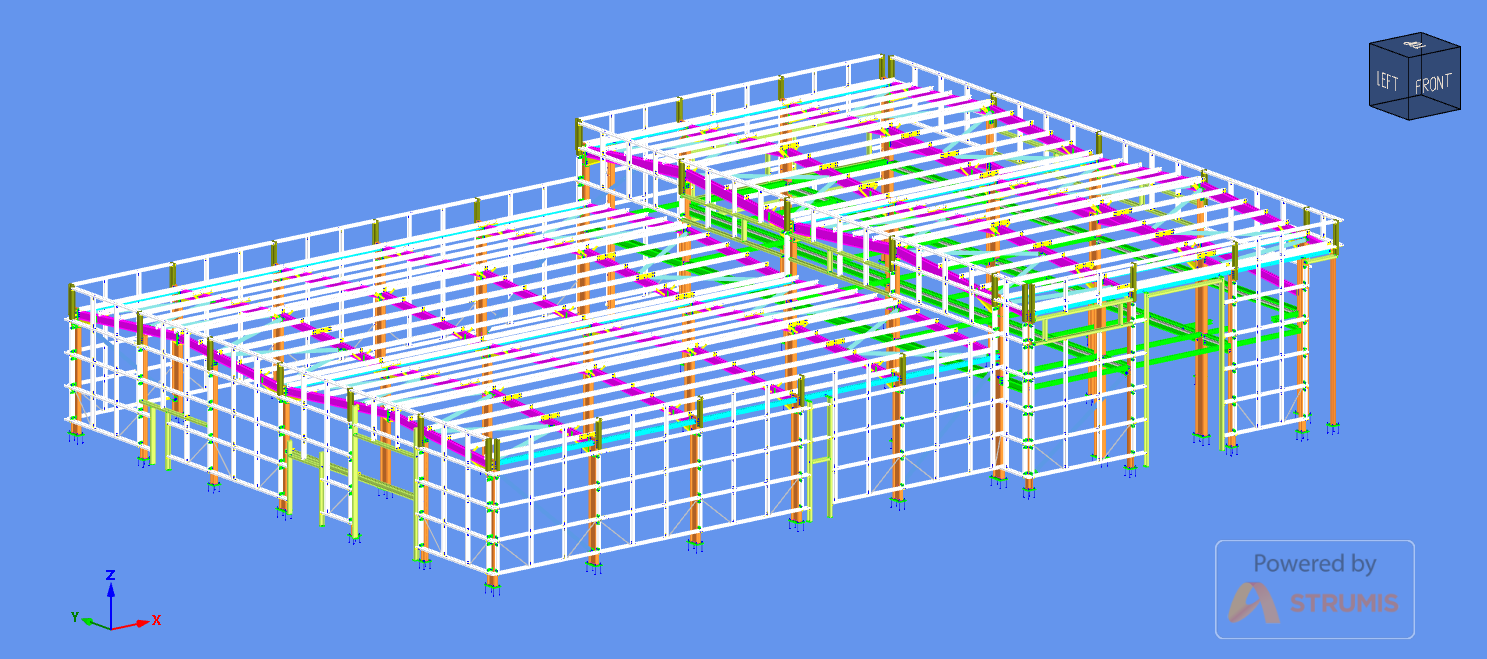
\includegraphics[width=1.0\linewidth]{a3img/1.png}
	\caption{Complete Model}
	\label{fig:ass3img1}
\end{figure}

\begin{figure}
	\centering
	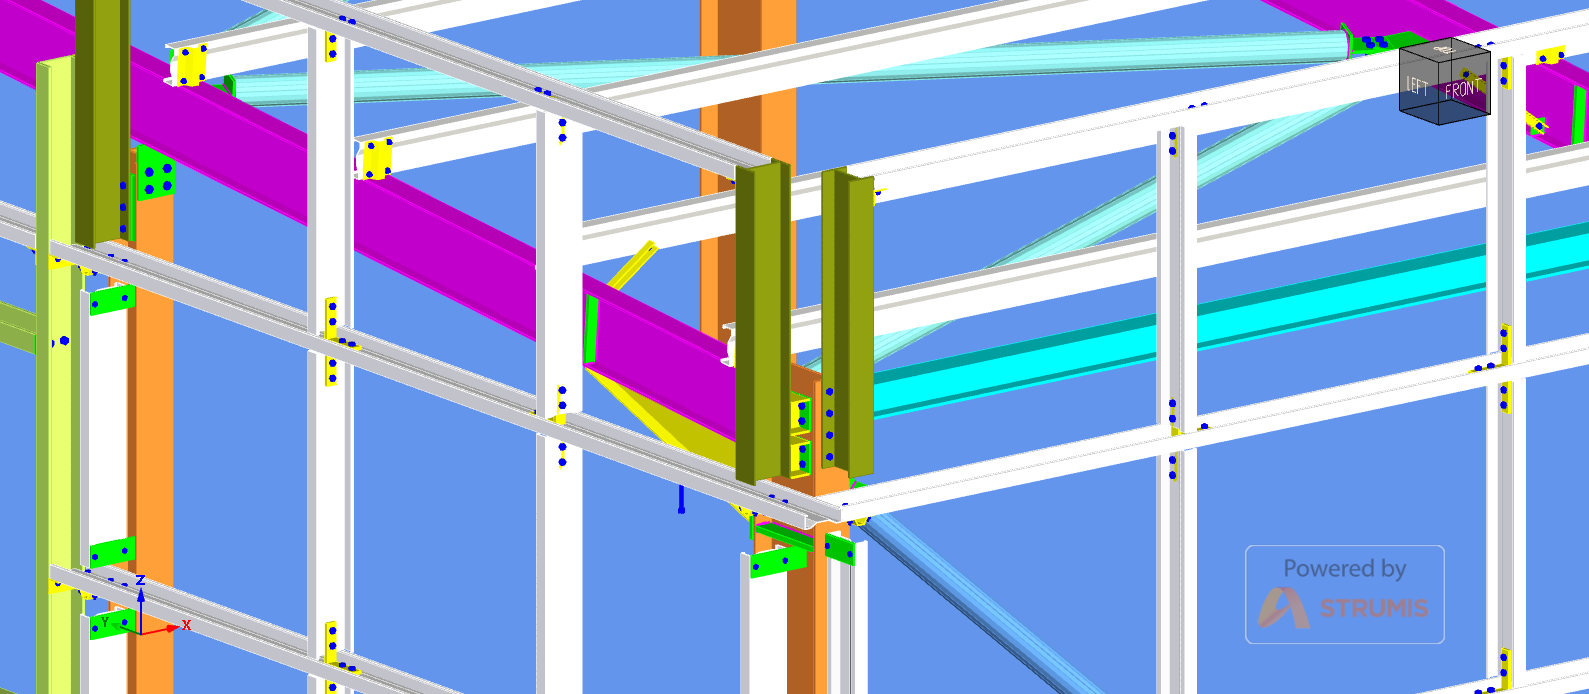
\includegraphics[width=1.0\linewidth]{a3img/2.png}
	\caption{Cladding Framing}
	\label{fig:ass3img2}
\end{figure}

\begin{figure}
	\centering
	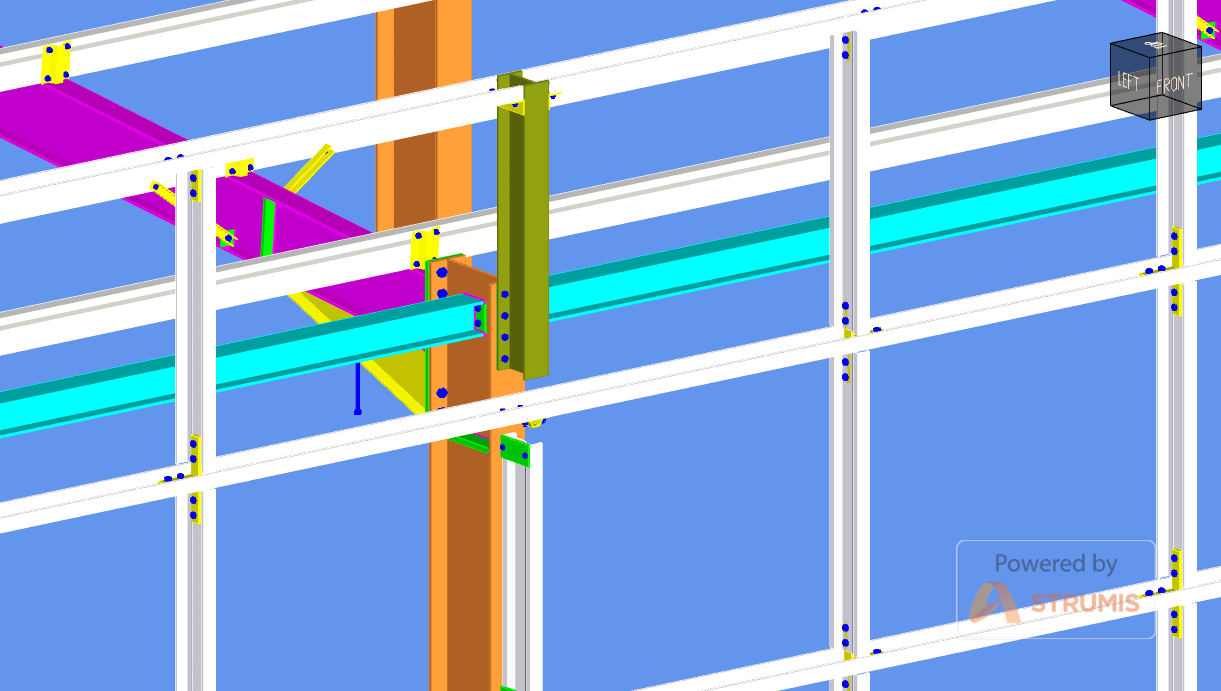
\includegraphics[width=1.0\linewidth]{a3img/3.png}
	\caption{Cladding Framing}
	\label{fig:ass3img3}
\end{figure}

\begin{figure}
	\centering
	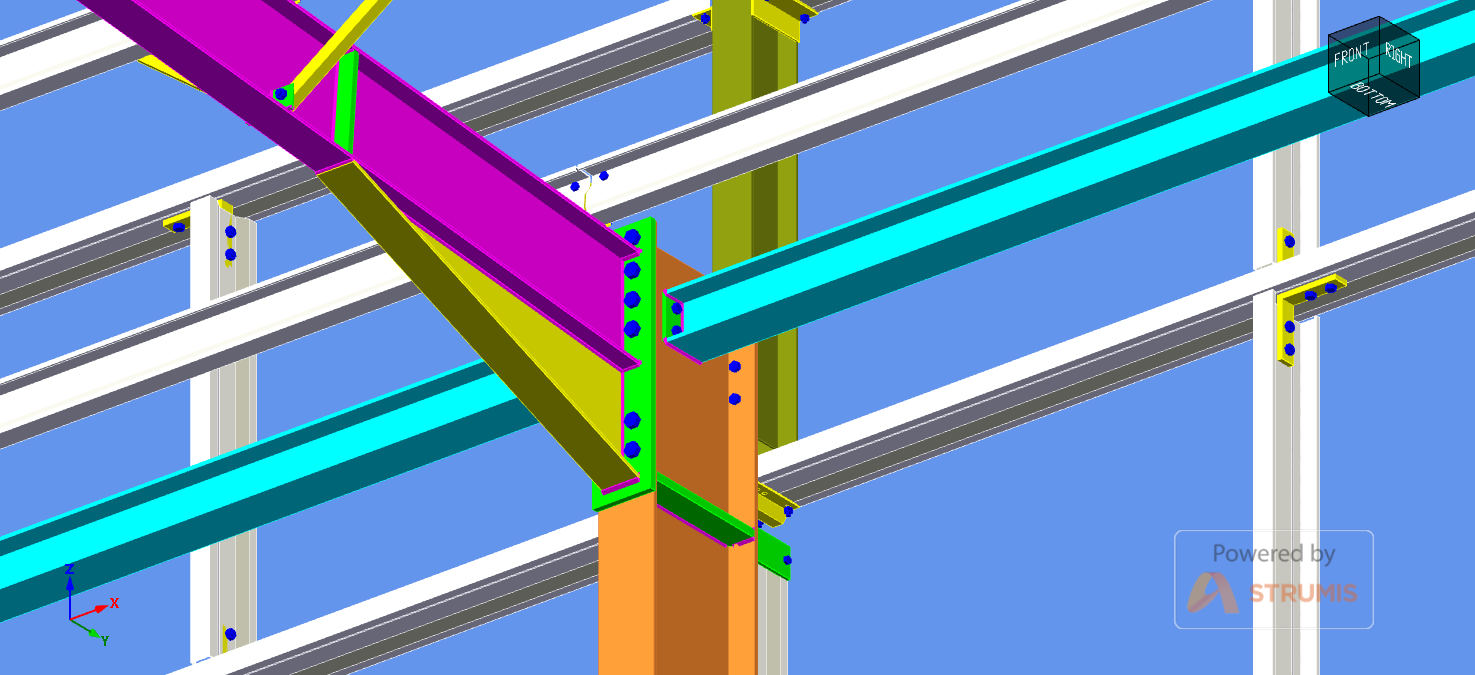
\includegraphics[width=1.0\linewidth]{a3img/4.png}
	\caption{Roof Beam to Column Connection}
	\label{fig:ass3img4}
\end{figure}

\begin{figure}
	\centering
	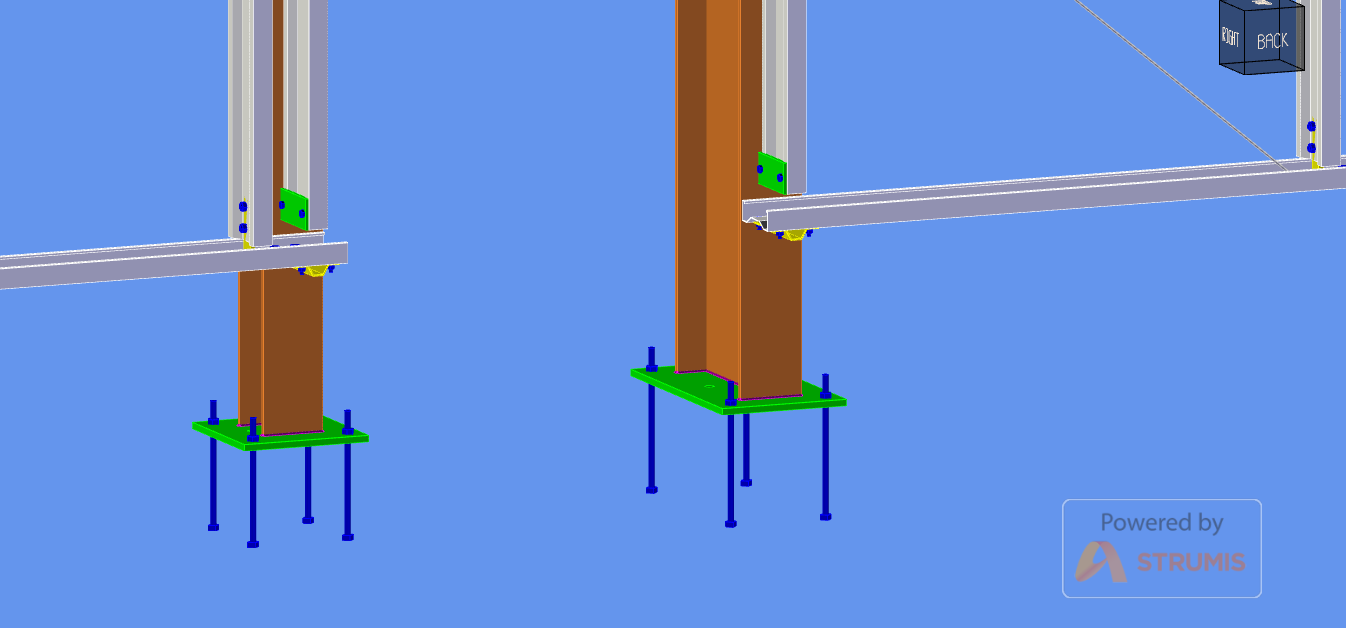
\includegraphics[width=1.0\linewidth]{a3img/5.png}
	\caption{Anchor Bolts}
	\label{fig:ass3img5}
\end{figure}

\begin{figure}
	\centering
	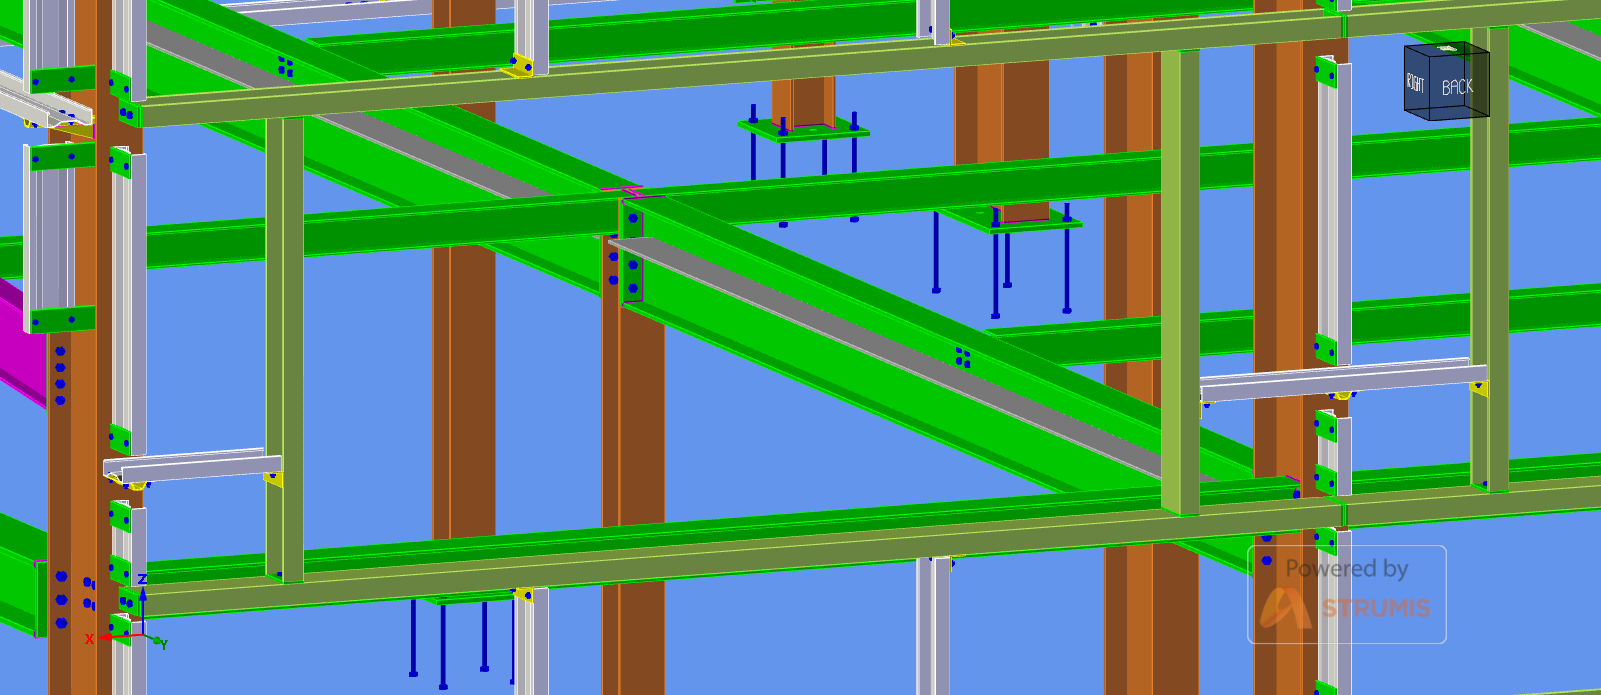
\includegraphics[width=1.0\linewidth]{a3img/6.png}
	\caption{Precast Conc Support Beams}
	\label{fig:ass3img6}
\end{figure}

\begin{figure}
	\centering
	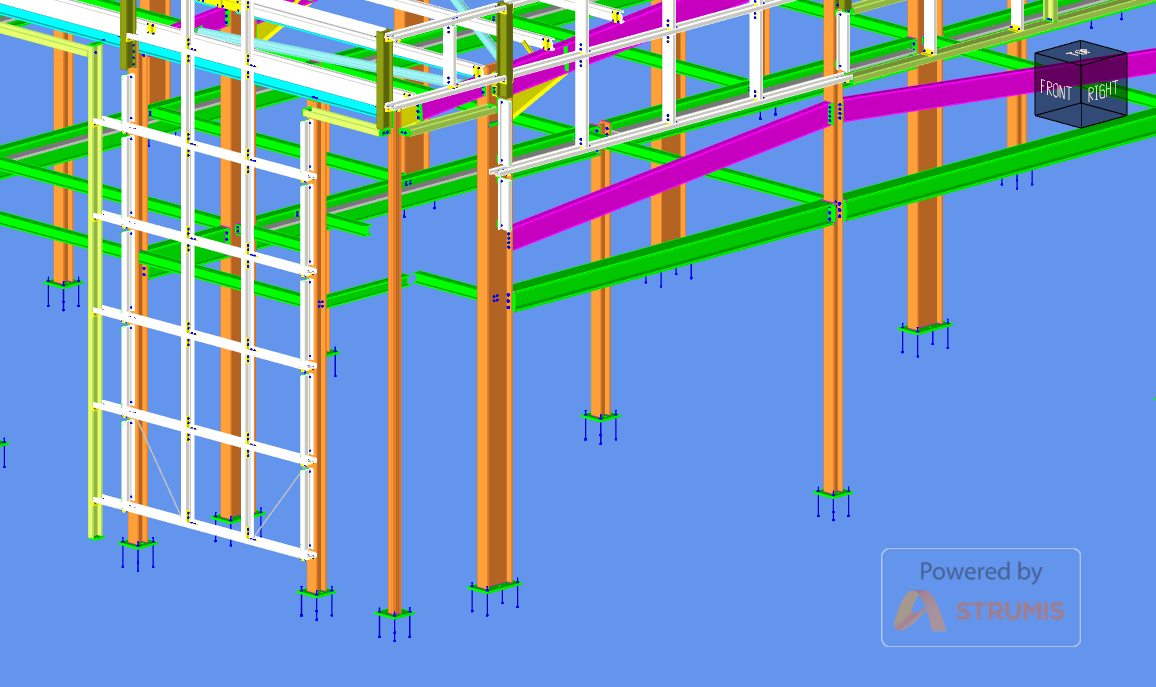
\includegraphics[width=1.0\linewidth]{a3img/7.png}
	\caption{Corner Image}
	\label{fig:ass3img7}
\end{figure}

\begin{figure}
	\centering
	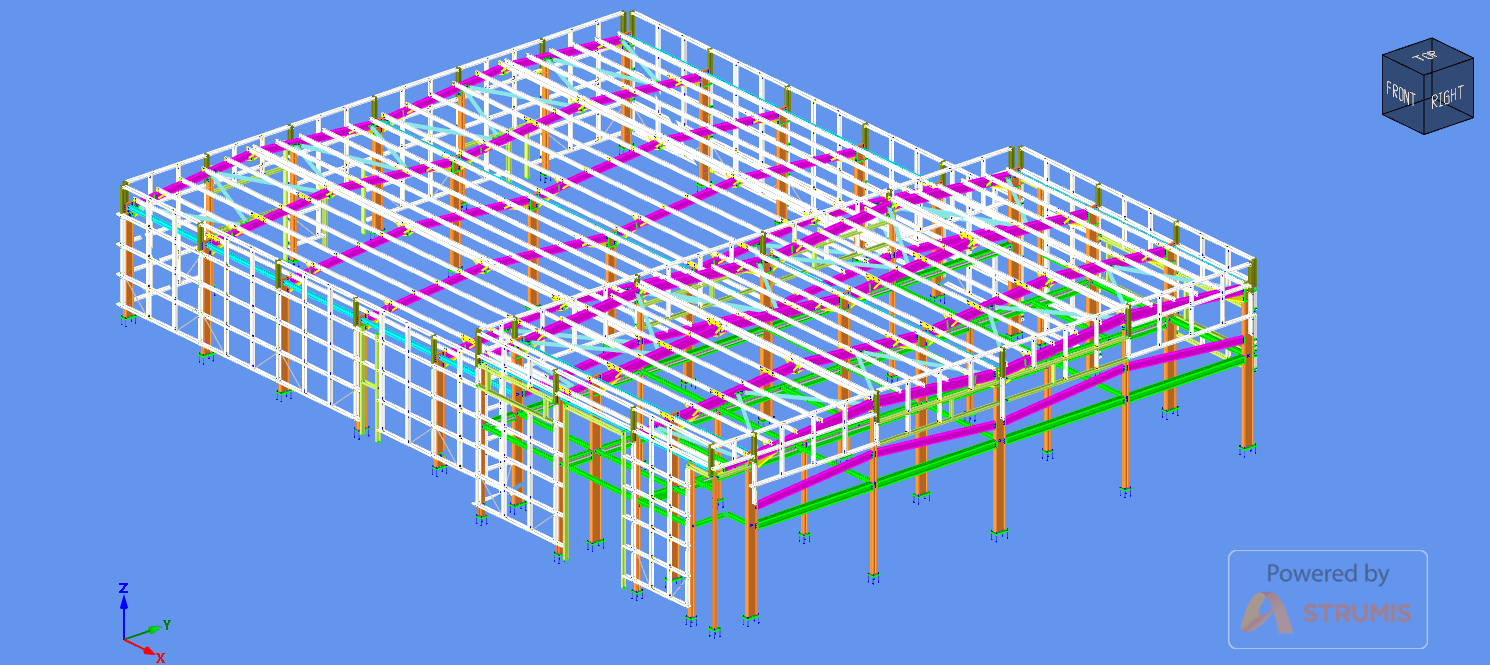
\includegraphics[width=1.0\linewidth]{a3img/8.png}
	\caption{Model Image (Reverse Angle)}
	\label{fig:ass3img8}
\end{figure}

\begin{figure}
	\centering
	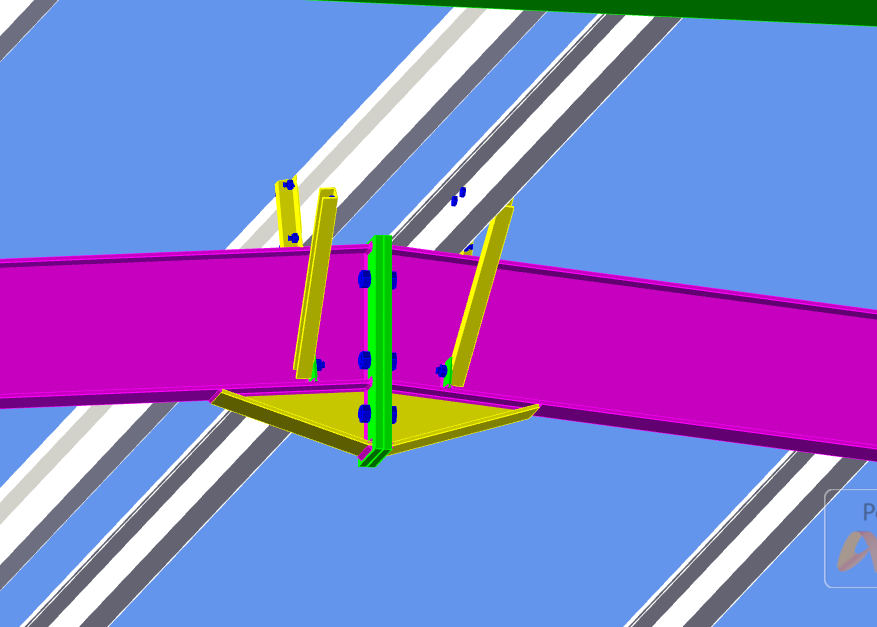
\includegraphics[width=1.0\linewidth]{a3img/9.png}
	\caption{Apex Joint}
	\label{fig:ass3img9}
\end{figure}

\newpage


\textbf{Submission}\\
Your completed assignment comprising of a single zip archive of all Revit files is to be uploaded to Moodle on or before the date and time indicated.  

\vspace{0.5cm}

\textbf{Late Submission}\\
Failure to submit your assignment on or before the date and time indicated on Moodle will result in a penalty of 5\% per day or part thereof.

\vspace{0.5cm}
\textbf{Marking Scheme}

\begin{table}[h!]
     \begin{center}
     \begin{tabular}{p{9cm}  p{2cm} }
     \toprule
      \textbf\large{Element} & \textbf\large{Proportion} \\ 
    \cmidrule(r){1-1}\cmidrule(lr){2-2}
    	Detailed Revit Model of the Steel Framed Structure 		 	& 50\%\\
    	Detailed General Arrangement Drawings 						& 10\%\\
        Rebar Drawings 												& 10\%\\
        Detailed Steelwork Drawings, including Connection Details 	& 10\%\\
        Framing Schedule (provided on A1 drawing) 					& 10\%\\
        Moodle Forum participation				 					& 10\%\\    
      \\ \bottomrule
      \end{tabular}
      \label{tbl:markSchemeAsmt3}
      \end{center}
 \end{table}

\end{document}